\documentclass[10pt]{article}
\usepackage[left=1.5cm, right=1.5cm, top=0.8in, bottom=0.7in]{geometry}
\usepackage{fancyhdr}
\pagestyle{fancy}
\usepackage{lastpage}
\usepackage[most,breakable]{tcolorbox}
\usepackage{pdfcol,xcolor}
\usepackage{tikz}
\usepackage[linesnumbered,ruled,vlined]{algorithm2e}
%\usepackage{url}
\usepackage{dsfont}
\usepackage{amssymb,amsmath}
\usepackage{xspace}
\usepackage[normalem]{ulem}
\usepackage{bm}
\usepackage{enumitem}
\usepackage[breaklinks=true,colorlinks,linkcolor=magenta,urlcolor=magenta,citecolor=black]{hyperref}
\usepackage{cleveref}
\usepackage{xpatch}
\xpretocmd{\algorithm}{\hsize=\linewidth}{}{}

\newtcolorbox[auto counter]{exercise}[1][]{%
	colback=yellow!10,colframe=red!75!black,coltitle=white,use color stack,enforce breakable,enhanced,fonttitle=\bfseries,before upper={\parindent15pt\noindent}, title={\color{white}Exercise~\thetcbcounter: #1}}
\pagecolor{yellow!10}

\lhead{\textbf{University of Waterloo}}
\rhead{\textbf{2024 Spring}}
\chead{\textbf{CS480/680}}
\rfoot{\thepage/\pageref*{LastPage}}
\cfoot{\textbf{Yao-Liang Yu (yaoliang.yu@uwaterloo.ca) \textcopyright 2024}}

\newcommand{\pf}{\mathfrak{p}}
\newcommand{\qf}{\mathfrak{q}}
\newcommand{\pb}{\bar{p}}
\newcommand{\qb}{\bar{q}}
\newcommand{\pfb}{\bar{\mathfrak{p}}}
\newcommand{\qfb}{\bar{\mathfrak{q}}}
\newcommand{\rK}{\reflectbox{\ensuremath{K}}}
\newcommand{\lb}{\mathtt{lb}}
\newcommand{\ub}{\mathtt{ub}}
\newcommand{\mi}{\mathtt{maxiter}}
\newcommand{\tol}{\mathtt{tol}}
\newcommand{\softmax}{\mathsf{softmax}}
\newcommand{\KL}{\mathsf{KL}}

\newcommand{\bv}{\mathbf{b}}
\newcommand{\ev}{\mathbf{e}}
\newcommand{\fv}{\mathbf{f}}
\newcommand{\gv}{\mathbf{g}}
\newcommand{\pv}{\mathbf{p}}
\newcommand{\qv}{\mathbf{q}}
\newcommand{\rv}{\mathbf{r}}
\newcommand{\uv}{\mathbf{u}}
\newcommand{\wv}{\mathbf{w}}
\newcommand{\xv}{\mathbf{x}}
\newcommand{\yv}{\mathbf{y}}
\newcommand{\zv}{\mathbf{z}}
\newcommand{\gbs}{\bm{\mathsf{g}}}
\newcommand{\wbs}{\bm{\mathsf{w}}}
\newcommand{\xbs}{\bm{\mathsf{x}}}
\newcommand{\Xv}{\mathbf{X}}
\newcommand{\Yv}{\mathbf{Y}}
\newcommand{\Bsf}{\mathsf{B}}
\newcommand{\Lsf}{\mathsf{L}}
\newcommand{\Usf}{\mathsf{U}}
\newcommand{\Xsf}{\mathsf{X}}
\newcommand{\Ysf}{\mathsf{Y}}
\newcommand{\Zsf}{\mathsf{Z}}
\newcommand{\Dc}{\mathcal{D}}
\newcommand{\Nc}{\mathcal{N}}
\newcommand{\EE}{\mathds{E}}
\newcommand{\RR}{\mathds{R}}
\newcommand{\alphav}{\boldsymbol{\alpha}}
\newcommand{\betav}{\boldsymbol{\beta}}
\newcommand{\epsilonv}{\boldsymbol{\epsilon}}
\newcommand{\gammav}{\boldsymbol{\gamma}}

\newcommand{\ans}[1]{{\color{blue}\textsf{Ans}: #1}}
\newcommand{\argmin}{\mathop{\mathrm{argmin}}}
\newcommand{\argmax}{\mathop{\mathrm{argmax}}}
\newcommand{\diag}{\mathrm{diag}}
\newcommand{\dinner}[2]{\langle\!\langle#1,#2\rangle\!\rangle}
\newcommand{\inner}[2]{\langle #1, #2 \rangle}
\newcommand{\one}{\mathbf{1}}
\newcommand{\pred}[1]{[\![#1]\!]}
\newcommand{\prox}[1]{\mathrm{P}_{#1}}
\newcommand{\sgm}{\mathsf{sgm}}
\newcommand{\sign}{\mathop{\mathrm{sign}}}
\newcommand{\tr}{\mathrm{tr}}
\newcommand{\zero}{\mathbf{0}}

\newcommand{\ea}{{et al.}\xspace}
\newcommand{\eg}{{e.g.}\xspace}
\newcommand{\ie}{{i.e.}\xspace}
\newcommand{\iid}{{i.i.d.}\xspace}
\newcommand{\cf}{{cf.}\xspace}
\newcommand{\wrt}{{w.r.t.}\xspace}
\newcommand{\aka}{{a.k.a.}\xspace}
\newcommand{\etc}{{etc.}\xspace}

\newcommand{\red}[1]{{\color{red}#1}}
\newcommand{\blue}[1]{{\color{blue}#1}}
\newcommand{\magenta}[1]{{\color{magenta}#1}}
\newcommand{\green}[1]{{\color{green}#1}}
%===========================================================
\begin{document}

\begin{center}
	\large{\textbf{CS480/680: Introduction to Machine Learning} \\ Homework 4\\ \red{Due: 11:59 pm, July 24, 2024}, \red{submit on LEARN}.} \\

	{\bf \green{NAME}} \\
	{\bf \green{student number}}

\end{center}

\begin{center}
	Submit your writeup in pdf and all source code in a zip file (with proper documentation). Write a script for each programming exercise so that the TA can easily run and verify your results. Make sure your code runs!

	[Text in square brackets are hints that can be ignored.]
\end{center}

\begin{exercise}[Generative Adversarial Networks (10 pts)]
	Please follow the instructions of this \href{https://cs.uwaterloo.ca/~y328yu/mycourses/480/a4-wgan.ipynb}{\texttt{ipynb} file}.

	\begin{enumerate}
		\item (2+6 pts) Complete the missing coding parts in the provided \href{https://cs.uwaterloo.ca/~y328yu/mycourses/480/a4-wgan.ipynb}{\texttt{ipynb} file}.

		\item (1 pt) Visualization of the loss:

		      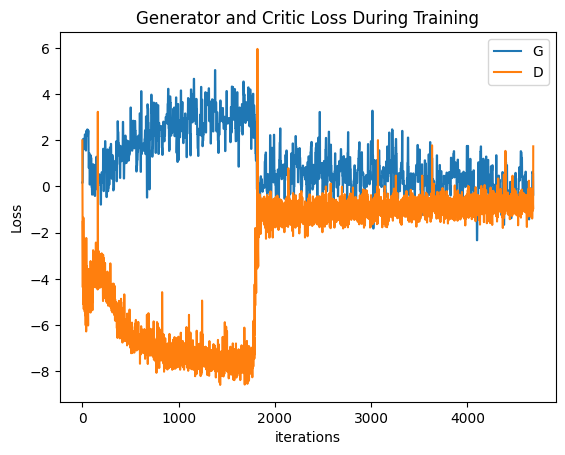
\includegraphics[width=.45\textwidth]{plot/ex1/loss.png}

		\item (1 pt) Visualization of the final generated images:

		      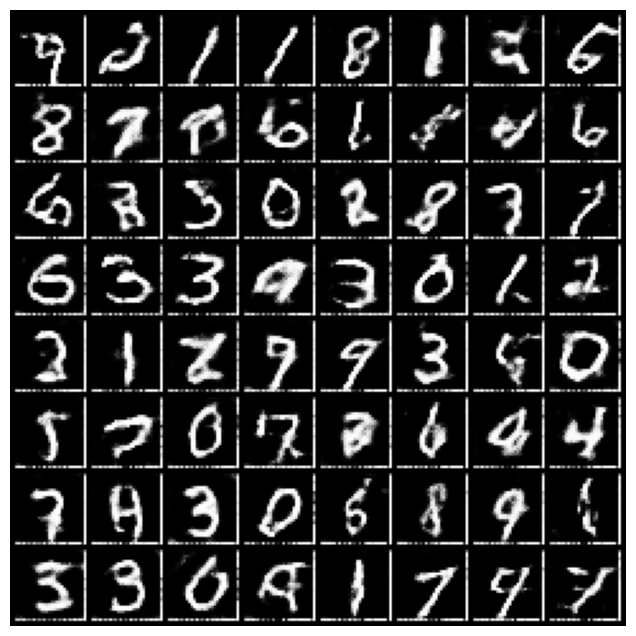
\includegraphics[width=.45\textwidth]{plot/ex1/generation.png}
	\end{enumerate}
\end{exercise}



\begin{exercise}[Quantile and push-forward (8 pts)]
	In this exercise we compute and simulate the push-forward map $T$ that transforms a reference density $r$ into a target density $p$. Recall that the quantile function of a (univariate) random variable $\Xsf$ is defined as the inverse of its cumulative distribution function (cdf) $F$:
	\begin{align}
		F(x) = \Pr(\Xsf \leq x), \qquad
		Q(u) = F^{-1}(u),~~ u \in \red{(}0,1 \red{)}.
	\end{align}
	We assume $F$ is continuous and strictly increasing so that $Q^{-1} = F$. A nice property of the quantile function, relevant to sampling, is that if $\Usf \sim \mathrm{Uniform}(0,1)$, then $Q(\Usf) \sim F$.

	In the following, do not confuse \href{https://en.wikipedia.org/wiki/Cumulative_distribution_function}{cdf} (signaled by uppercase letters) with \href{https://en.wikipedia.org/wiki/Probability_density_function}{pdf} (\ie, density, signaled by lowercase letters).

	\begin{enumerate}
		\item (1 pt) Consider the Gaussian mixture model (GMM) with density $p(x) = \red{\tfrac{\lambda}{\sigma_1}} \varphi\left( \frac{x-\mu_1}{\sigma_1}\right) + \red{\tfrac{1-\lambda}{\sigma_2}} \varphi\left( \frac{x-\mu_2}{\sigma_2}\right)$, where $\varphi$ is the \emph{density} of the standard normal distribution (mean 0 and variance 1). Implement the following to create a dataset of $n=1000$ samples from the GMM $p$:
		      \begin{itemize}
			      \item Sample $\Usf_i\sim \mathrm{Uniform}(0,1)$.
			      \item If $\Usf_i < \lambda$, sample $\Xsf_i \sim \mathcal{N}(\mu_1, \sigma_1^{2})$; otherwise sample $\Xsf_i \sim \mathcal{N}(\mu_2, \sigma_2^{2})$.
		      \end{itemize}
		      \uline{Plot the histogram} of the generated $\Xsf_i$ (with $b=50$ bins) and submit your script as \\ \verb|X = GMMsample(gmm, n=1000, b=50), gmm.lambda=0.5, gmm.mu=[1,-1], gmm.sigma=[0.5,0.5]|

		      [See \href{https://pythonspot.com/matplotlib-histogram/}{here} or \href{https://realpython.com/python-histograms/}{here} for how to plot a histogram in \verb|matplotlib| or \verb|pandas| (or \verb|numpy| if you insist).]

		      \ans

		      \includegraphics[width=.5\textwidth]{plot/ex2/GMMsample.png}

		\item (2 pts) Compute $\Usf_i = \Phi^{-1}\big(F(\Xsf_i))$, where $F$ is the \emph{cdf} of the GMM in Ex 2.1 and $\Phi$ is the \emph{cdf} of standard normal. \uline{Plot the histogram} of the generated $\Usf_i$ (with $b$ bins). From your inspection, what distribution should $\Usf_i$ follow (approximately)? Submit your script as \verb|GMMinv(X, gmm, b=50)|.

		      [This \href{https://docs.scipy.org/doc/scipy/reference/generated/scipy.special.erf.html}{page} may be helpful.]

		      \ans

		      $\Usf_i$ follows a standard normal distribution.\\
		      \includegraphics[width=.5\textwidth]{plot/ex2/GMMinv.png}

		\item (2 pts) Let $\Zsf \sim \mathcal{N}(0,1)$. We now compute the push-forward map $T$ so that $T(\Zsf) = \Xsf \sim p$ (the GMM in Ex 2.1). We use the formula:
		      \begin{align}
			      T(z) = Q( \Phi(z) ),
		      \end{align}
		      where $\Phi$ is the \emph{cdf} of the standard normal distribution and $Q = F^{-1}$ is the quantile function of $\Xsf$, namely the GMM $p$ in Ex 2.1. \uline{Implement the following binary search} \Cref{alg:bs} to numerically compute $T$. \uline{Plot the function $T$ with input $z \in [-5,5]$ (increment 0.1)}. \uline{Submit your main script} as \verb|BinarySearch(F, u, lb=-100, ub=100, maxiter=100, tol=1e-5)|, where \verb|F| is a function. You may need to write another script to compute and plot $T$ (based on \verb|BinarySearch|).

		      \begin{algorithm}[H]
			      \DontPrintSemicolon
			      \KwIn{$u\in(0,1)$, \red{$\lb  < 0 <  \ub$}, $\mi, \tol$}

			      \KwOut{$x$ such that $|F(x) - u| \leq \tol$}

			      \While(\tcp*[f]{lower bound too large}){$F(\lb) > u$}{
				      $\ub \gets \lb$

				      $\lb \gets 2 * \lb$
			      }

			      \While(\tcp*[f]{upper bound too small}){$F(\ub) < u$}{
				      $\lb \gets \ub$

				      $\ub \gets 2 * \ub$
			      }

			      \For{$i=1, \ldots, \mi$ }{

				      $x \gets \tfrac{\lb+\ub}{2}$ \tcp*{try middle point}

				      $t \gets F(x)$


				      \If{ $t > u$}{$\ub \gets x$}
				      \Else{$\lb \gets x$}

				      \If{$ |t - u| \leq \tol $}{\textbf{break}}

			      }

			      \caption{Binary search for solving a monotonic nonlinear equation $F(x) = u$.}
			      \label{alg:bs}
		      \end{algorithm}

		      \ans

		      \includegraphics[width=.5\textwidth]{plot/ex2/T.png}

		\item (2 pts) Sample (independently) $\Zsf_i \sim \mathcal{N}(0,1), i = 1, \ldots, n=1000$ and let $\tilde \Xsf_i = T(\Zsf_i)$, where $T$ is computed by your \verb|BinarySearch|. \uline{Plot the histogram of the generated $\tilde \Xsf_i$} (with $b$ bins) and \uline{submit your script} as \verb|PushForward(Z, gmm)|. Is the histogram similar to the one in Ex 2.1?

		      \ans

		      Yes, they are very similar\\
		      \includegraphics[width=.5\textwidth]{plot/ex2/PushForward.png}

		\item (1 pt) Now let us compute $\tilde \Usf_i = \Phi^{-1}\big(F(\tilde \Xsf_i))$ as in Ex 2.2, with $\tilde \Xsf_i$'s being generated in Ex 2.4. \uline{Plot the histogram of the resulting $\tilde \Usf_i$} (with $b$ bins). From your inspection what distribution should $\tilde \Usf_i$ follow (approximately)? [No need to submit any script, as you can recycle \verb|GMMinv|.]

		      \ans

		      $\tilde \Usf_i$ follows a standard normal distribution.\\
		      \includegraphics[width=.5\textwidth]{plot/ex2/tilde_U.png}
	\end{enumerate}

\end{exercise}


\end{document}
